% answers.tex —— 1977 年·新疆卷（文科） · 参考答案与详细解析片段
% 由 tools/generate_projects.py 依来源总账自 1977/1977_数学真题_新疆文_试题.md + 1977/1977_数学真题_新疆文_解析正文.md + 1977/1977_数学真题_新疆文_答案要点.md 生成，勿手改（改源 MD 后重跑）


\begin{gktip}
固定源是题面与解答连续出现的解答汇编材料。下文逐题独立推导，并对照源解答复算关键结论；第 3 题源卷的 b、d 形近排印之误与第 6 题源解答的一处排印错位在相应题下留注。
\end{gktip}

\begin{answer}
\gksolhead{1}{}

\textbf{题目}（15 分）：

\Needspace{5\baselineskip}
解方程：

\nopagebreak[4]
\[
\frac{x-1}{x+1}-\frac{5}{1-x}=\frac{4}{x^2-1}
\]

\Needspace{4\baselineskip}
\textbf{解析}

\Needspace{5\baselineskip}
方程有意义的条件是分母不为零，即 $x\ne\pm1$。注意到 $1-x=-(x-1)$、$x^2-1=(x-1)(x+1)$，去分母得

\nopagebreak[4]
\[
(x-1)^2+5(x+1)=4,
\]

\Needspace{5\baselineskip}
即

\nopagebreak[4]
\[
x^2-2x+1+5x+5=4,
\qquad
x^2+3x+2=0.
\]

\Needspace{5\baselineskip}
分解因式，

\nopagebreak[4]
\[
(x+2)(x+1)=0,
\qquad
x=-2\ \text{\text{或}}\ x=-1.
\]

检验：$x=-1$ 使分母 $x+1$ 为零，是增根，舍去；$x=-2$ 代入原方程，左端为 $3-\dfrac53=\dfrac43$，右端为 $\dfrac{4}{(-3)(-1)}=\dfrac43$，等式成立。故原方程的根为 $x=-2$。

\gkanswer{答案：$x=-2$。}

\end{answer}
\begin{answer}
\gksolhead{2}{}

\textbf{题目}（16 分）：

红心大队贫下中农坚决顶住“四人帮”对农业学大寨运动的干扰和破坏，积极发展养猪事业，1974 年底全大队养猪 200 头，到 1976 年底发展到 1200 头，求平均每年的增长率，（精确到 $1\%$）

\Needspace{4\baselineskip}
\textbf{解析}

\Needspace{5\baselineskip}
设平均每年的增长率为 $x$。1974 年底到 1976 年底经过两年，依题意

\nopagebreak[4]
\[
200(1+x)^2=1200,
\]

\Needspace{5\baselineskip}
即

\nopagebreak[4]
\[
(1+x)^2=6,
\qquad
1+x=\pm\sqrt6.
\]

\Needspace{5\baselineskip}
解得

\nopagebreak[4]
\[
x_1=\sqrt6-1\approx1.45=145\%,
\qquad
x_2=-\sqrt6-1\approx-3.45.
\]

$x_2$ 为负值，不合题意，舍去。由 $\sqrt6\approx2.449$，$x_1\approx1.449$，精确到 $1\%$ 即 $145\%$，故平均每年的增长率为 $145\%$。

\gkanswer{答案：平均每年的增长率为 $145\%$。}

\end{answer}
\begin{answer}
\gksolhead{3}{}

\textbf{题目}：

计算：

\Needspace{5\baselineskip}
（1） 化简：（7 分）

\nopagebreak[4]
\[
\frac{\frac{3}{4}(ab)^{-\frac{1}{3}}\left(\frac{4}{9}a^4b^{\frac{2}{3}}\right)^{\frac{1}{2}}}{2a^3\sqrt{a^2}}
\]

\begin{gktip}
\textbf{源注}：原卷括号内该因式印作“$a^4d^{\frac{2}{3}}$”，源解答按 $a^4b^{\frac{2}{3}}$ 展开计算——字母 $b$ 与前一因式 $(ab)^{-\frac{1}{3}}$ 一致，且恰使化简结果中 $b$ 的指数归零，系 $b$、$d$ 形近排印之误，本卷按 $b$ 转录。
\end{gktip}

（2） 已知 $\lg 2=0.3010$，求 $\lg\sqrt{800}$（7 分）

\Needspace{4\baselineskip}
\textbf{解析}

\gksubpart{（1）}

\Needspace{5\baselineskip}
先把括号内的因式化为幂：

\nopagebreak[4]
\[
\left(\frac49a^4b^{\frac23}\right)^{\frac12}
=\left(\frac49\right)^{\frac12}a^{4\times\frac12}b^{\frac23\times\frac12}
=\frac23\,a^2\,b^{\frac13},
\]

\Needspace{5\baselineskip}
且分母中 $\sqrt{a^2}=a^{2\times\frac12}=a$。代入原式，

\nopagebreak[4]
\[
\begin{aligned}
\text{\text{原式}}
&=\frac{\frac34\,a^{-\frac13}b^{-\frac13}\cdot\frac23\,a^2b^{\frac13}}{2a^3\cdot a}\\
&=\frac{\frac34\cdot\frac23}{2}\cdot a^{-\frac13+2-3-1}\cdot b^{-\frac13+\frac13}\\
&=\frac14\,a^{-\frac73}
=\frac{\sqrt[3]{a^2}}{4a^3}.
\end{aligned}
\]

\begin{gktip}
\textbf{源注}：原卷题面该因式印作“$a^4d^{\frac{2}{3}}$”，源解答按 $a^4b^{\frac{2}{3}}$ 展开计算，判定为 $b$、$d$ 形近排印之误，题面已按 $b$ 转录。又，源解答倒数第二行末尾多印一个字母 $b$（无指数），而其后的续行即为 $\dfrac{\sqrt[3]{a^2}}{4a^3}$，且该行 $b$ 的指数和恰为零（$b^0=1$），故判定该 $b$ 为排印残留，化简结果不含 $b$。
\end{gktip}

\gksubpart{（2）}

\nopagebreak[4]
\[
\begin{aligned}
\lg\sqrt{800}
&=\lg\sqrt{2^3\times10^2}
=\lg10+\frac32\lg2\\
&=1+\frac32\times0.3010
=1.4515.
\end{aligned}
\]

\gkanswer{答案（1）：$\dfrac{\sqrt[3]{a^2}}{4a^3}$。}

\gkanswer{答案（2）：$1.4515$。}

\end{answer}
\begin{answer}
\gksolhead{4}{}

\textbf{题目}（16 分）：

求证：四边形对边中点的连线互相平分。

\begin{gktip}
原源 PDF 第 3 页附有四边形及对边中点连线示意图；LaTeX 版按源图重绘。
\end{gktip}
\nopagebreak[4]
\begin{center}% 1977 年新疆卷（文科）第四题：四边形 ABCD，E、F、M、N 分别为 AD、AB、BC、CD 的中点，
% 实线 EM 与 FN，虚线 EF、FM、MN、NE 及对角线 BD（按源卷第 3 页布局：A 左上、D 右上、B 左下、C 右下）
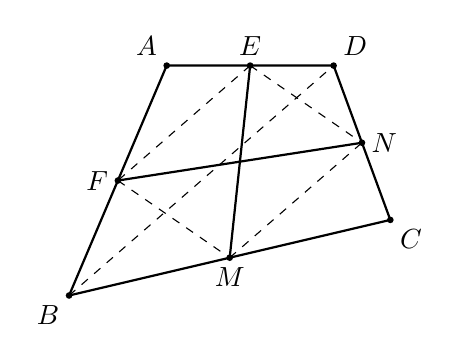
\begin{tikzpicture}[scale=1.0]
  \coordinate (B) at (0,0);
  \coordinate (A) at (1.24,2.92);
  \coordinate (D) at (3.36,2.92);
  \coordinate (C) at (4.08,0.96);
  \coordinate (E) at (2.30,2.92);
  \coordinate (F) at (0.62,1.46);
  \coordinate (M) at (2.04,0.48);
  \coordinate (N) at (3.72,1.94);
  \draw[thick] (A)--(D)--(C)--(B)--cycle;
  \draw[thick] (E)--(M);
  \draw[thick] (F)--(N);
  \draw[dashed] (E)--(F);
  \draw[dashed] (E)--(N);
  \draw[dashed] (F)--(M);
  \draw[dashed] (M)--(N);
  \draw[dashed] (B)--(D);
  \fill (A) circle (1.2pt) node[above left] {$A$};
  \fill (D) circle (1.2pt) node[above right] {$D$};
  \fill (C) circle (1.2pt) node[below right] {$C$};
  \fill (B) circle (1.2pt) node[below left] {$B$};
  \fill (E) circle (1.2pt) node[above] {$E$};
  \fill (F) circle (1.2pt) node[left] {$F$};
  \fill (M) circle (1.2pt) node[below] {$M$};
  \fill (N) circle (1.2pt) node[right] {$N$};
\end{tikzpicture}
\end{center}
\nopagebreak[4]
\Needspace{4\baselineskip}
\textbf{解析}

设四边形 $ABCD$，$E$、$F$、$M$、$N$ 分别为边 $AD$、$AB$、$BC$、$CD$ 的中点，求证的是 $EM$ 与 $FN$ 互相平分。分别连 $FM$、$MN$、$NE$、$EF$ 及对角线 $BD$：
\nopagebreak[4]
\begin{center}% 1977 年新疆卷（文科）第四题：四边形 ABCD，E、F、M、N 分别为 AD、AB、BC、CD 的中点，
% 实线 EM 与 FN，虚线 EF、FM、MN、NE 及对角线 BD（按源卷第 3 页布局：A 左上、D 右上、B 左下、C 右下）
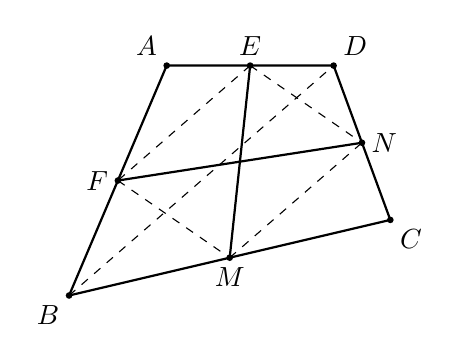
\begin{tikzpicture}[scale=1.0]
  \coordinate (B) at (0,0);
  \coordinate (A) at (1.24,2.92);
  \coordinate (D) at (3.36,2.92);
  \coordinate (C) at (4.08,0.96);
  \coordinate (E) at (2.30,2.92);
  \coordinate (F) at (0.62,1.46);
  \coordinate (M) at (2.04,0.48);
  \coordinate (N) at (3.72,1.94);
  \draw[thick] (A)--(D)--(C)--(B)--cycle;
  \draw[thick] (E)--(M);
  \draw[thick] (F)--(N);
  \draw[dashed] (E)--(F);
  \draw[dashed] (E)--(N);
  \draw[dashed] (F)--(M);
  \draw[dashed] (M)--(N);
  \draw[dashed] (B)--(D);
  \fill (A) circle (1.2pt) node[above left] {$A$};
  \fill (D) circle (1.2pt) node[above right] {$D$};
  \fill (C) circle (1.2pt) node[below right] {$C$};
  \fill (B) circle (1.2pt) node[below left] {$B$};
  \fill (E) circle (1.2pt) node[above] {$E$};
  \fill (F) circle (1.2pt) node[left] {$F$};
  \fill (M) circle (1.2pt) node[below] {$M$};
  \fill (N) circle (1.2pt) node[right] {$N$};
\end{tikzpicture}
\end{center}
\nopagebreak[4]
\Needspace{5\baselineskip}
在 $\triangle BCD$ 中，$M$、$N$ 分别为 $BC$、$CD$ 的中点，由三角形中位线定理，

\nopagebreak[4]
\[
MN\parallel BD,
\qquad
MN=\frac12BD.
\]

\Needspace{5\baselineskip}
同理，在 $\triangle DAB$ 中，$E$、$F$ 分别为 $AD$、$AB$ 的中点，

\nopagebreak[4]
\[
EF\parallel BD,
\qquad
EF=\frac12BD.
\]

故 $EF\parallel MN$ 且 $EF=MN$。有一组对边平行而且相等的四边形是平行四边形，所以四边形 $FMNE$ 是平行四边形；平行四边形的对角线互相平分，而 $EM$ 与 $FN$ 正是平行四边形 $FMNE$ 的两条对角线，故 $EM$ 与 $FN$ 互相平分。

\gkanswer{答案：见解析版}

\end{answer}
\begin{answer}
\gksolhead{5}{}

\textbf{题目}（10 分）：

\Needspace{5\baselineskip}
解方程组

\nopagebreak[4]
\[
\begin{cases}
2x-3y=9\\
3x+4y=5
\end{cases}
\]

\Needspace{4\baselineskip}
\textbf{解析}

\Needspace{5\baselineskip}
将第一个方程两边乘 $3$，第二个方程两边乘 $2$，再相减以消去 $x$：

\nopagebreak[4]
\[
(2x-3y)\times3-(3x+4y)\times2=9\times3-5\times2,
\]

\Needspace{5\baselineskip}
即

\nopagebreak[4]
\[
6x-9y-6x-8y=27-10,
\qquad
-17y=17,
\]

\Needspace{5\baselineskip}
所以 $y=-1$。代入第一个方程，

\nopagebreak[4]
\[
2x-3\times(-1)=9,
\qquad
x=3.
\]

方程组的解为 $x=3$、$y=-1$。

\gkanswer{答案：$x=3$，$y=-1$。}

\end{answer}
\begin{answer}
\gksolhead{6}{}

\textbf{题目}（14 分）：

红升人民公社小水库拦水坝的横断面为梯形，坝顶宽 2.5 米，坝高 4 米，迎水坡、背水坡与水平面的夹角分别是 $30^\circ$ 和 $45^\circ$，求坝底的宽。（精确到 $0.1$ 米）

\begin{gktip}
原源 PDF 第 4 页附有拦水坝横断面示意图，坝顶标有 2.5 的尺寸标注，左侧绘有水面示意短线；LaTeX 版按源图重绘。
\end{gktip}
\nopagebreak[4]
\begin{center}% 1977 年新疆卷（文科）第六题：拦水坝梯形横断面 ABCD（AD 为坝顶，BC 为坝底），
% AE、DF 为坝高的垂线（虚线），左侧水面示意短线，角 B=30°、角 C=45°，
% 坝顶上方标 2.5 尺寸线（按源卷第 4 页布局；比例约 1:2.2，非严格尺寸）
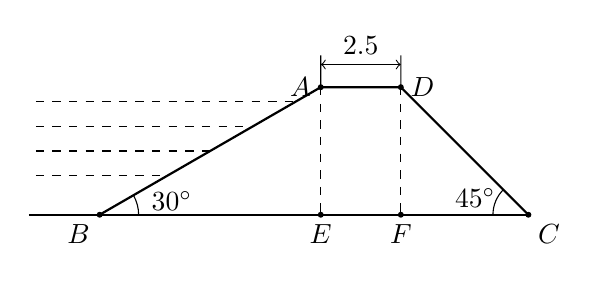
\begin{tikzpicture}[scale=0.9]
  \coordinate (B) at (0,0);
  \coordinate (E) at (3.12,0);
  \coordinate (F) at (4.25,0);
  \coordinate (C) at (6.05,0);
  \coordinate (A) at (3.12,1.8);
  \coordinate (D) at (4.25,1.8);
  \draw[thick] (-1.0,0)--(C);
  \draw[thick] (B)--(A)--(D)--(C);
  \draw[dashed] (A)--(E);
  \draw[dashed] (D)--(F);
  % 水面示意短线（迎水坡一侧）
  \draw[dashed] (-0.9,0.55)--(0.95,0.55);
  \draw[dashed] (-0.9,0.90)--(1.56,0.90);
  \draw[dashed] (-0.9,1.25)--(2.17,1.25);
  \draw[dashed] (-0.9,1.60)--(2.77,1.60);
  % 坝顶 2.5 尺寸标注
  \draw[thin] (A)--(3.12,2.25);
  \draw[thin] (D)--(4.25,2.25);
  \draw[<->] (3.12,2.12)--(4.25,2.12) node[midway,above] {$2.5$};
  % 角标注
  \draw (0.55,0) arc[start angle=0,end angle=30,radius=0.55];
  \node at (1.02,0.20) {$30^\circ$};
  \draw ([shift={(180:0.5)}]C) arc[start angle=180,end angle=135,radius=0.5];
  \node at (5.30,0.24) {$45^\circ$};
  \fill (A) circle (1.2pt) node[left] {$A$};
  \fill (D) circle (1.2pt) node[right] {$D$};
  \fill (B) circle (1.2pt) node[below left] {$B$};
  \fill (E) circle (1.2pt) node[below] {$E$};
  \fill (F) circle (1.2pt) node[below] {$F$};
  \fill (C) circle (1.2pt) node[below right] {$C$};
\end{tikzpicture}
\end{center}
\nopagebreak[4]
\Needspace{4\baselineskip}
\textbf{解析}

\Needspace{5\baselineskip}
分别由 $A$、$D$ 向 $BC$ 作垂线，垂足为 $E$、$F$，则

\nopagebreak[4]
\[
AE=DF=4.
\]

\Needspace{5\baselineskip}
在直角三角形 $ABE$ 中，$\angle B=30^\circ$，

\nopagebreak[4]
\[
BE=AE\cdot\cot30^\circ=4\sqrt3\ \text{（\text{米}）},
\]

\Needspace{5\baselineskip}
在直角三角形 $DCF$ 中，$\angle C=45^\circ$，

\nopagebreak[4]
\[
CF=DF\cdot\cot45^\circ=4\ \text{（\text{米}）}.
\]

\Needspace{5\baselineskip}
又 $EF=AD=2.5$ 米，所以

\nopagebreak[4]
\[
BC=4\sqrt3+4+2.5\approx13.4\ \text{（\text{米}）}.
\]

故坝底宽约为 $13.4$ 米。
\nopagebreak[4]
\begin{center}% 1977 年新疆卷（文科）第六题：拦水坝梯形横断面 ABCD（AD 为坝顶，BC 为坝底），
% AE、DF 为坝高的垂线（虚线），左侧水面示意短线，角 B=30°、角 C=45°，
% 坝顶上方标 2.5 尺寸线（按源卷第 4 页布局；比例约 1:2.2，非严格尺寸）
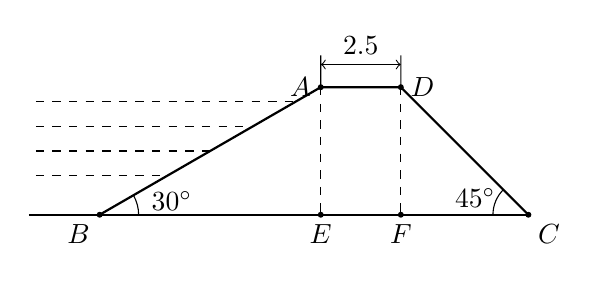
\begin{tikzpicture}[scale=0.9]
  \coordinate (B) at (0,0);
  \coordinate (E) at (3.12,0);
  \coordinate (F) at (4.25,0);
  \coordinate (C) at (6.05,0);
  \coordinate (A) at (3.12,1.8);
  \coordinate (D) at (4.25,1.8);
  \draw[thick] (-1.0,0)--(C);
  \draw[thick] (B)--(A)--(D)--(C);
  \draw[dashed] (A)--(E);
  \draw[dashed] (D)--(F);
  % 水面示意短线（迎水坡一侧）
  \draw[dashed] (-0.9,0.55)--(0.95,0.55);
  \draw[dashed] (-0.9,0.90)--(1.56,0.90);
  \draw[dashed] (-0.9,1.25)--(2.17,1.25);
  \draw[dashed] (-0.9,1.60)--(2.77,1.60);
  % 坝顶 2.5 尺寸标注
  \draw[thin] (A)--(3.12,2.25);
  \draw[thin] (D)--(4.25,2.25);
  \draw[<->] (3.12,2.12)--(4.25,2.12) node[midway,above] {$2.5$};
  % 角标注
  \draw (0.55,0) arc[start angle=0,end angle=30,radius=0.55];
  \node at (1.02,0.20) {$30^\circ$};
  \draw ([shift={(180:0.5)}]C) arc[start angle=180,end angle=135,radius=0.5];
  \node at (5.30,0.24) {$45^\circ$};
  \fill (A) circle (1.2pt) node[left] {$A$};
  \fill (D) circle (1.2pt) node[right] {$D$};
  \fill (B) circle (1.2pt) node[below left] {$B$};
  \fill (E) circle (1.2pt) node[below] {$E$};
  \fill (F) circle (1.2pt) node[below] {$F$};
  \fill (C) circle (1.2pt) node[below right] {$C$};
\end{tikzpicture}
\end{center}
\nopagebreak[4]
\begin{gktip}
\textbf{源注}：源解答在印有「BE＝AE ctg30°」一行的下一行印作「4＝√3（米）」，按本题几何关系应为「＝4√3（米）」的排印错位——$\cot30^\circ=\sqrt3$，$BE=4\sqrt3\approx6.93$，且源解答末行 $BC=4\sqrt3+4+2.5=13.4$（米）正以此为准。本文按 $4\sqrt3$ 计算。
\end{gktip}

\gkanswer{答案：坝底宽约为 $13.4$ 米。}

\end{answer}
\begin{answer}
\gksolhead{7}{}

\textbf{题目}（15 分）：

已知，直线过 $A(2,-5)$ 和 $B(-3,0)$ 两点，求此直线方程，并指出直线的斜率 $K$=？，直线与 $OX$ 轴正方向的夹角 $\alpha$=？

\begin{gktip}
原源 PDF 第 5 页解答旁附有坐标系与直线示意图；LaTeX 版按源图重绘并移至题面处。
\end{gktip}
\nopagebreak[4]
\begin{center}% 1977 年新疆卷（文科）第七题：直线 y=-x-3 过 B(-3,0) 与 A(2,-5) 的坐标系示意图，
% 两轴带箭头，坐标轴上绘单位刻度点（按源卷第 5 页布局）
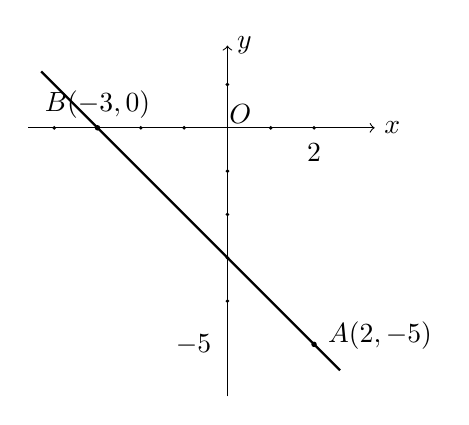
\begin{tikzpicture}[scale=0.55]
  \draw[->] (-4.6,0)--(3.4,0) node[right] {$x$};
  \draw[->] (0,-6.2)--(0,1.9) node[right] {$y$};
  \node at (0.30,0.32) {$O$};
  % 单位刻度点
  \foreach \xx in {-4,-2,-1,1,2} \fill (\xx,0) circle (1.3pt);
  \foreach \yy in {1,-1,-2,-3,-4} \fill (0,\yy) circle (1.3pt);
  \node[below] at (2,-0.15) {$2$};
  \node[left] at (-0.15,-5) {$-5$};
  % 直线 y=-x-3
  \draw[thick] (-4.3,1.3)--(2.6,-5.6);
  \fill (-3,0) circle (1.8pt) node[above] {$B(-3,0)$};
  \fill (2,-5) circle (1.8pt);
  \node[right] at (2.1,-4.8) {$A(2,-5)$};
\end{tikzpicture}
\end{center}
\nopagebreak[4]
\Needspace{4\baselineskip}
\textbf{解析}

\Needspace{5\baselineskip}
由 $A(2,-5)$、$B(-3,0)$ 两点，直线 $AB$ 的方程用两点式写出：

\nopagebreak[4]
\[
\frac{y-0}{-5-0}=\frac{x-(-3)}{2-(-3)},
\]

\Needspace{5\baselineskip}
即

\nopagebreak[4]
\[
\frac{y}{-5}=\frac{x+3}{5},
\qquad
5y=-5x-15,
\]

\Needspace{5\baselineskip}
化简得

\nopagebreak[4]
\[
y=-x-3.
\]
\nopagebreak[4]
\begin{center}% 1977 年新疆卷（文科）第七题：直线 y=-x-3 过 B(-3,0) 与 A(2,-5) 的坐标系示意图，
% 两轴带箭头，坐标轴上绘单位刻度点（按源卷第 5 页布局）
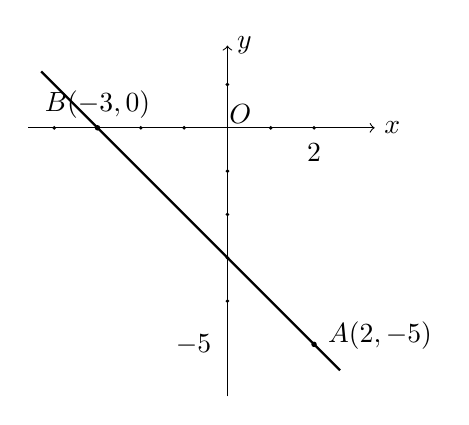
\begin{tikzpicture}[scale=0.55]
  \draw[->] (-4.6,0)--(3.4,0) node[right] {$x$};
  \draw[->] (0,-6.2)--(0,1.9) node[right] {$y$};
  \node at (0.30,0.32) {$O$};
  % 单位刻度点
  \foreach \xx in {-4,-2,-1,1,2} \fill (\xx,0) circle (1.3pt);
  \foreach \yy in {1,-1,-2,-3,-4} \fill (0,\yy) circle (1.3pt);
  \node[below] at (2,-0.15) {$2$};
  \node[left] at (-0.15,-5) {$-5$};
  % 直线 y=-x-3
  \draw[thick] (-4.3,1.3)--(2.6,-5.6);
  \fill (-3,0) circle (1.8pt) node[above] {$B(-3,0)$};
  \fill (2,-5) circle (1.8pt);
  \node[right] at (2.1,-4.8) {$A(2,-5)$};
\end{tikzpicture}
\end{center}
\nopagebreak[4]
\Needspace{5\baselineskip}
所以斜率 $K=-1$。设直线与 $OX$ 轴正方向的夹角为 $\alpha$（$0^\circ\le\alpha<180^\circ$），则 $\tan\alpha=K=-1$，故

\nopagebreak[4]
\[
\alpha=135^\circ.
\]

\gkanswer{答案：$y=-x-3$；$K=-1$；$\alpha=135^\circ$。}

\end{answer}